% Energy Fingerprints — Energy Data Hackdays 2026 pitch deck
% Replace all values marked TBD before presenting.
\documentclass[10pt,aspectratio=169]{beamer}

\usepackage[T1]{fontenc}
% `sourcesans` is the maintained TeX package for the Source Sans Pro family.
% Medium copy and Black display text make the type system visibly intentional.
\usepackage[default,medium,black,scale=1.03]{sourcesans}
\usepackage{tikz}
\usetikzlibrary{arrows.meta,positioning,calc,fit}

% Springer Nature Elements palette: blue-led, with restrained teal/orange accents.
\definecolor{ink}{HTML}{01324B}
\definecolor{inksoft}{HTML}{025E8D}
\definecolor{paper}{HTML}{F8F8F8}
\definecolor{muted}{HTML}{555555}
\definecolor{mint}{HTML}{00A69D}
\definecolor{sun}{HTML}{F58220}
\definecolor{blue}{HTML}{0070A8}
\definecolor{rose}{HTML}{BE1818}
\definecolor{line}{HTML}{DADADA}

\setbeamercolor{normal text}{fg=ink,bg=paper}
\setbeamercolor{frametitle}{fg=ink,bg=paper}
\setbeamercolor{title}{fg=paper}
\setbeamercolor{subtitle}{fg=mint}
\setbeamercolor{structure}{fg=blue}
\setbeamercolor{alerted text}{fg=rose}
\setbeamercolor{footline}{fg=muted,bg=paper}
\usefonttheme{professionalfonts}
\setbeamerfont{title}{family=\sffamily,series=\bfseries,size=\fontsize{28}{32}}
\setbeamerfont{subtitle}{family=\sffamily,size=\large}
\setbeamerfont{frametitle}{family=\sffamily,series=\bfseries,size=\fontsize{19}{23}}
\setbeamerfont{normal text}{family=\sffamily,size=\small}
\setbeamertemplate{navigation symbols}{}
\setbeamertemplate{itemize items}[circle]
\setbeamersize{text margin left=0.9cm,text margin right=0.9cm}
\setbeamertemplate{footline}{\hfill\insertshorttitle\quad\textcolor{line}{|}\quad\insertframenumber/\inserttotalframenumber\hspace{0.9cm}\vspace{0.25cm}}
\setbeamertemplate{frametitle}{\vspace{0.35cm}\insertframetitle\par\vspace{0.18cm}\textcolor{mint}{\rule{1.1cm}{1.3pt}}\vspace{0.18cm}}
\setlength{\leftmargini}{1em}

\newcommand{\tagline}[1]{\tikz[baseline=(tag.base)]\node[rounded corners=2pt,fill=mint!18,text=ink,inner xsep=5pt,inner ysep=2pt,font=\sffamily\scriptsize\bfseries] (tag) {#1};}
\newcommand{\placeholder}[1]{\tikz[baseline=(tag.base)]\node[rounded corners=2pt,draw=muted!45,dashed,text=muted,inner xsep=5pt,inner ysep=2pt,font=\scriptsize] (tag) {TBD: #1};}
\newcommand{\metric}[2]{\begin{tikzpicture}[baseline]
  \node[fill=ink,rounded corners=2pt,minimum width=2.2cm,minimum height=1.05cm,text width=1.85cm,align=left,inner sep=7pt,text=paper] {\textcolor{mint}{\sffamily\small\bfseries #1}\\[-1pt]\sffamily\scriptsize #2};
\end{tikzpicture}}

% #1 TP, #2 FN, #3 FP, #4 TN. Keep all four on the same held-out split.
\newcommand{\confusionmatrix}[4]{%
\tikz[x=0.92cm,y=0.62cm,baseline=(current bounding box.north)]{
  \node[font=\scriptsize\bfseries,text=muted] at (1,3.25) {PREDICTED};
  \node[font=\scriptsize] at (0.5,2.82) {Asset};
  \node[font=\scriptsize] at (1.5,2.82) {No asset};
  \node[font=\scriptsize\bfseries,text=muted,rotate=90] at (-0.72,1.45) {ACTUAL};
  \node[font=\scriptsize] at (-0.05,2.05) {Asset};
  \node[font=\scriptsize] at (-0.12,0.85) {No asset};
  \node[fill=mint!32,minimum width=.92cm,minimum height=.62cm,align=center] at (.5,2.05) {\scriptsize TP\\\bfseries #1};
  \node[fill=sun!35,minimum width=.92cm,minimum height=.62cm,align=center] at (1.5,2.05) {\scriptsize FN\\\bfseries #2};
  \node[fill=rose!28,minimum width=.92cm,minimum height=.62cm,align=center] at (.5,.85) {\scriptsize FP\\\bfseries #3};
  \node[fill=blue!20,minimum width=.92cm,minimum height=.62cm,align=center] at (1.5,.85) {\scriptsize TN\\\bfseries #4};
}}
% #1 width, #2 the rule in words, #3 headline metrics, #4 the caveat.
% Flat: a single accent rule at the left edge, no box, per DESIGN_PREFERENCES.
% Built from plain LaTeX boxes rather than a TikZ node -- a node with `text width`
% sets its own paragraph and spaces words far more loosely than body copy.
\newsavebox{\rbbox}
\newcommand{\rulebaseline}[4]{\par\smallskip\noindent
\sbox{\rbbox}{\parbox{#1}{\raggedright
  {\sffamily\scriptsize\bfseries\color{blue}RULE BASELINE}\\[2.5pt]
  {\sffamily\footnotesize\color{ink}#2}\\[3pt]
  {\sffamily\scriptsize\bfseries\color{ink}#3}\\[1.5pt]
  {\sffamily\scriptsize\color{muted}#4}}}%
\textcolor{mint}{\rule[-\dp\rbbox]{1.4pt}{\dimexpr\ht\rbbox+\dp\rbbox\relax}}%
\hspace{7pt}\usebox{\rbbox}\par\smallskip}
\newcommand{\confusiontable}[6]{%
\scriptsize\renewcommand{\arraystretch}{1.35}\setlength{\tabcolsep}{3pt}%
\begin{tabular}{@{}lrr@{}}
\textbf{Actual cohort} & \textbf{Flagged} & \textbf{Not flagged} \\\hline
#1 & #3 & #4 \\
#2 & #5 & #6 \\
\end{tabular}}

\title{Energy Fingerprints}
\subtitle{Make the invisible energy system visible}
\author{newspaper}
\institute{Energy Data Hackdays 2026 \enspace | \enspace AEW Energie}
\date{[TBD: pitch date]}
\newcommand{\decktitle}{Energy Fingerprints}
\titlegraphic{}

\begin{document}

{\setbeamercolor{background canvas}{bg=ink}
\begin{frame}[plain]
  \vspace{1.05cm}
  {\color{mint}\sffamily\large\bfseries ENERGY DATA HACKDAYS 2026}\par\vspace{0.35cm}
  {\color{paper}\sffamily\fontsize{34}{40}\selectfont\bfseries Energy Fingerprints}\par\vspace{0.25cm}
  {\color{mint}\sffamily\Large Make the invisible energy system visible.}\par\vspace{0.85cm}
  {\color{paper}\large From 15-minute smart-meter data to explainable household asset intelligence.}\par\vfill
  {\color{paper}\small newspaper \hfill AEW Energie challenge}
\end{frame}}

\begin{frame}{The grid sees one number. We reveal the causes.}
\begin{columns}[T,onlytextwidth]
\column{.52\textwidth}
\large A household's net load hides the assets that shape flexibility, infrastructure demand, and solar potential.
\vspace{0.45cm}
\begin{itemize}\itemsep0.45em
  \item 4 years of anonymised, 15-minute readings
  \item $\sim$90k households; $\sim$1k labelled customers
  \item Privacy-preserving: no appliance sensors, no customer intervention
\end{itemize}
\column{.43\textwidth}
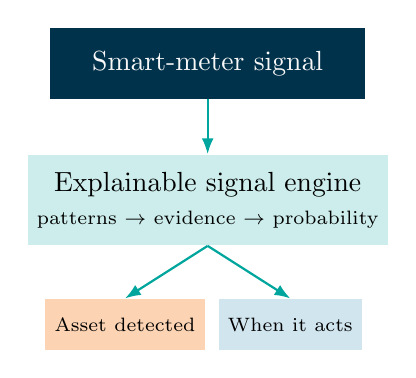
\begin{tikzpicture}[node distance=7mm]
  \node[fill=ink,text=paper,minimum width=4.0cm,minimum height=.9cm,align=center] (meter) {Smart-meter signal};
  \node[below=of meter,fill=mint!20,minimum width=4.0cm,minimum height=1.15cm,align=center] (engine) {Explainable signal engine\\\scriptsize patterns $\rightarrow$ evidence $\rightarrow$ probability};
  \node[fill=sun!34,minimum width=1.7cm,minimum height=.65cm,align=center,font=\scriptsize] (asset) at ($(engine.south)+(-1.05cm,-1.0cm)$) {Asset detected};
  \node[fill=blue!18,minimum width=1.7cm,minimum height=.65cm,align=center,font=\scriptsize] (activity) at ($(engine.south)+(1.05cm,-1.0cm)$) {When it acts};
  \draw[-{Latex[length=2mm]},thick,mint] (meter)--(engine);
  \draw[-{Latex[length=2mm]},thick,mint] (engine.south)--(asset.north);
  \draw[-{Latex[length=2mm]},thick,mint] (engine.south)--(activity.north);
\end{tikzpicture}
\end{columns}
\end{frame}

\begin{frame}{One interpretable workflow, five asset lenses}
\begin{center}
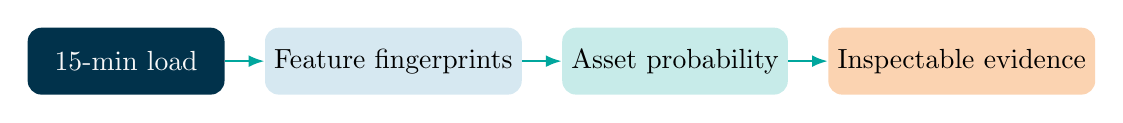
\begin{tikzpicture}[node distance=5mm]
  \node[fill=ink,rounded corners=5pt,text=paper,minimum width=2.5cm,minimum height=.85cm,align=center] (a) {15-min load};
  \node[right=of a,fill=blue!16,rounded corners=5pt,minimum width=2.5cm,minimum height=.85cm,align=center] (b) {Feature fingerprints};
  \node[right=of b,fill=mint!22,rounded corners=5pt,minimum width=2.5cm,minimum height=.85cm,align=center] (c) {Asset probability};
  \node[right=of c,fill=sun!35,rounded corners=5pt,minimum width=2.5cm,minimum height=.85cm,align=center] (d) {Inspectable evidence};
  \draw[-{Latex[length=2mm]},thick,mint] (a)--(b); \draw[-{Latex[length=2mm]},thick,mint] (b)--(c); \draw[-{Latex[length=2mm]},thick,mint] (c)--(d);
\end{tikzpicture}
\end{center}
\vspace{.5cm}
\begin{columns}[T,onlytextwidth]
\column{.28\textwidth}\tagline{EV}\par\small Sharp switch-on steps in grid import.
\column{.28\textwidth}\tagline{Heat pump}\par\small Cold-weather and persistent heating signatures.
\column{.28\textwidth}\tagline{Rooftop PV}\par\small Sunny-day midday import depression.
\end{columns}
\vspace{.35cm}
\begin{columns}[T,onlytextwidth]
\column{.28\textwidth}\tagline{Battery}\par\small Export displaced past solar noon.
\column{.28\textwidth}\tagline{Other devices}\par\small Repeated distinctive load motifs.
\column{.28\textwidth}\placeholder{demo evidence view}
\end{columns}
\end{frame}

\begin{frame}{EV: the model, and the rule it must beat}
\begin{columns}[T,onlytextwidth]
\column{.55\textwidth}
\tagline{E22 LIGHTGBM · HELD-OUT TEST}\par\vspace{.18cm}
\scriptsize 45 features, threshold frozen before the test was opened. Test (67 properties, 15 EV-labelled): \textbf{ROC-AUC 0.67}. Detects EV \emph{households}, not charging events.
\vspace{.10cm}
\rulebaseline{.52\textwidth}{Flag EV if grid import ever steps up by $\geq$\,9\,kW within one quarter-hour.}{\mbox{ROC-AUC 0.686}\enspace\mbox{F1 0.50}\enspace\mbox{n = 342}}{Threshold selected out-of-fold: 9.2\,kW in $\sim$100/100 grouped folds.}
\vspace{.04cm}
\scriptsize
\begin{itemize}\itemsep.04em
  \item The full plateau detector --- band, duration, edge --- scores 0.688: $\Delta$AUC \textbf{$-0.002$}\,$[-0.033,+0.029]$ over one line of $\max(\Delta P)$.
  \item \alert{$\sim$75\% of $\geq$9\,kW ramp days fall in Nov--Mar for EV owners \emph{and} non-owners.} Much of what every method here reads is winter heating, not charging.
\end{itemize}
\column{.40\textwidth}
\centering\scriptsize\textbf{LightGBM · held-out test}\\[2pt]
\confusiontable{\shortstack[l]{EV-labelled\\(GIGI)}}{\shortstack[l]{Unlabelled\\properties}}{10}{5}{20}{32}\\[2pt]
{\scriptsize\textcolor{muted}{$p \geq 0.392$; $n=67$.}}\\[8pt]
\textbf{Rule · 342 labelled samples}\\[2pt]
\confusiontable{\shortstack[l]{EV-labelled\\(GIGI)}}{\shortstack[l]{Unlabelled\\properties}}{49}{23}{75}{195}\\[2pt]
{\scriptsize\textcolor{muted}{Precision 0.40 is a \emph{floor}.}}
\end{columns}
\end{frame}

\begin{frame}{Heat-pump boiler: a physical detector, not a classifier}
\begin{columns}[T,onlytextwidth]
\column{.58\textwidth}
\tagline{WPB DETECTOR · LABEL-FREE}\par\vspace{.25cm}
\scriptsize The detector identifies heat-pump water-heater candidates from persistent plateaus in 15-minute grid-import data.
\vspace{.12cm}
\begin{itemize}\itemsep.10em
  \item p10 daily envelope: an event must recur on at least 90\% of days, rejecting irregular loads such as part-time EV charging.
  \item Plateau band: 0.25--1.2 kW for 1.5--9 h; it must recur in both January and July.
  \item Population sweep: 838 of 75,094 households flagged (1.1\%) as candidates.
  \item 4 labelled positives and 0 confirmed negatives: no confusion matrix or accuracy estimate.
\end{itemize}
\column{.37\textwidth}
\centering\textbf{Counterfactual recovery test}\\[3pt]
\metric{79.6\%}{Recovery at 0.3 kW injected}\par\vspace{.18cm}
\metric{94.2\%}{Recovery at 0.5 kW injected}\par\vspace{.18cm}
\small\textcolor{muted}{Synthetic events test sensitivity only; they do not establish precision.}
\end{columns}
\end{frame}

\begin{frame}{Rooftop PV: SolarPrint reads the solar imprint in demand}
\begin{columns}[T,onlytextwidth]
\column{.55\textwidth}
\tagline{HISTGRADIENTBOOSTING · 5-FOLD OOF}\par\vspace{.18cm}
\scriptsize 23 import-shape features; feed-in is used offline for silver labels, never as a feature. \textbf{GIGI ROC-AUC 0.92}.
\vspace{.10cm}
\rulebaseline{.52\textwidth}{Flag PV if the meter ever exported. You cannot inject what you do not generate.}{\mbox{F1 0.920}\enspace\mbox{recall 0.922}\enspace\mbox{n = 342}}{Zero tuned constants. A 0.2\,kW deadband changed 0 of 342 calls, so it was removed.}
\vspace{.04cm}
\scriptsize
\begin{itemize}\itemsep.04em
  \item Import-only variant --- midday draw $\div$ night draw --- scores \textbf{0.800} against a gradient-boosted model's 0.806 on the same samples.
  \item \alert{The rule's 23 false positives mostly \emph{have} PV}: median export 17.0\,kWh/day vs 19.6 for labelled PV homes; true negatives export exactly zero.
\end{itemize}
\column{.40\textwidth}
\centering\scriptsize\textbf{SolarPrint · population}\\[2pt]
\confusiontable{\shortstack[l]{GIGI PV\\(confirmed)}}{\shortstack[l]{Strictly\\unlabelled}}{260}{24}{4.6k}{65.6k}\\[2pt]
{\scriptsize\textcolor{muted}{$p \geq 0.5$; silver excluded.}}\\[8pt]
\textbf{Rule · 342 labelled samples}\\[2pt]
\confusiontable{\shortstack[l]{GIGI PV\\(confirmed)}}{\shortstack[l]{Unlabelled\\properties}}{259}{22}{23}{38}\\[2pt]
{\scriptsize\textcolor{muted}{Different denominators --- not\\comparable cell for cell.}}
\end{columns}
\end{frame}

\begin{frame}{Battery: a physical rule already reads storage}
\begin{columns}[T,onlytextwidth]
\column{.55\textwidth}
\rulebaseline{.52\textwidth}{Of the solar exported in the shoulder months, what share leaves the house \emph{after} solar noon?}{\mbox{ROC-AUC 0.855}\enspace\mbox{F1 0.892}\enspace\mbox{n = 242}}{Flag a battery above 0.50. Nothing here is fitted to the labels.}
\vspace{.08cm}
\scriptsize
\begin{itemize}\itemsep.04em
  \item \textbf{Why 0.50.} The sun is symmetric about noon: a home \emph{without} storage exports half before, half after. A battery eats the morning surplus and spills only once full. Non-battery homes measure 0.466, battery 0.561.
  \item \textbf{The trap we avoid.} 96\% of batteries sit in a PV home, so \texttt{has\_PV} alone scores 0.700 against battery. Every number here is measured \alert{within PV homes}, where \texttt{has\_PV} is worth 0.500.
\end{itemize}
\column{.40\textwidth}
\centering\scriptsize\textbf{Rule · 242 PV households}\\[2pt]
\confusiontable{\shortstack[l]{GIGI battery\\(confirmed)}}{\shortstack[l]{Unlabelled\\PV homes}}{170}{20}{21}{31}\\[2pt]
{\scriptsize\textcolor{muted}{Share after noon $\geq 0.50$. This is\\the rule baseline --- the trained\\PV-conditioned model is still to come.}}\\[7pt]
\textbf{The seasonal test}\\[1pt]
{\scriptsize\renewcommand{\arraystretch}{1.3}\setlength{\tabcolsep}{3pt}
\begin{tabular}{@{}lrr@{}}
 & \textbf{No batt.} & \textbf{Battery} \\\hline
Jun--Aug & 0.459 & 0.529 \\
Mar/Apr/Sep/Oct & 0.483 & \textbf{0.632} \\
\end{tabular}}\\[3pt]
{\scriptsize\textcolor{muted}{\textbf{Not west-facing roofs.} A battery\\saturates in high summer so the skew\\shrinks --- and it does, by 0.103.\\Non-battery homes move 0.024.\\A fixed roof cannot change azimuth.}}
\end{columns}
\end{frame}

\begin{frame}{Other-device classifier: turn unknown load shapes into leads}
\begin{columns}[T,onlytextwidth]
\column{.58\textwidth}
\tagline{OTHER DISTINCTIVE DEVICE}\par\vspace{.25cm}
\small The model flags repeated, unusual load motifs for review, then groups them into candidate device classes as labels mature.
\vspace{.18cm}
\begin{itemize}\itemsep.18em
  \item Input: recurring event shape, power, duration, timing, and seasonality
  \item Output: device-class probability or ``novel pattern'' candidate
  \item Evidence: a small set of representative events a human can inspect
\end{itemize}
\vspace{.12cm}\placeholder{cluster of recurring appliance signatures}
\column{.37\textwidth}
\centering\textbf{Evaluation placeholder}\\[4pt]
\confusiontable{\shortstack[l]{Asset present\\(TBD)}}{\shortstack[l]{Asset absent\\(TBD)}}{TBD}{TBD}{TBD}{TBD}\\[5pt]
\scriptsize\textcolor{muted}{Define the class and held-out split before reporting results.}
\end{columns}
\end{frame}

\begin{frame}{Trust is a feature, not a footnote}
\begin{columns}[T,onlytextwidth]
\column{.28\textwidth}\metric{Explainable}{Every score links to its evidence.}\par\vspace{.25cm}\small ``Why was this home flagged?'' has a visible answer.
\column{.28\textwidth}\metric{Honest}{Validation is held out and limitations stay visible.}\par\vspace{.25cm}\small We do not invent accuracy where labels are missing.
\column{.28\textwidth}\metric{Scalable}{One workflow can score the full population.}\par\vspace{.25cm}\small Designed for multi-year, 15-minute data.
\end{columns}
\vspace{.55cm}
\begin{center}\placeholder{insert one anonymised household evidence card here}\end{center}
\end{frame}

{\setbeamercolor{background canvas}{bg=ink}
\begin{frame}[plain]
  \vspace{1.2cm}\color{paper}
  {\sffamily\fontsize{30}{36}\selectfont\bfseries From meter data to better grid decisions.}\par\vspace{.35cm}
  {\color{mint}\sffamily\Large Asset intelligence, activity windows, and evidence---at population scale.}\par\vspace{.8cm}
  \begin{columns}[T,onlytextwidth]
  \column{.29\textwidth}\color{paper}\textbf{Forecasting}\\\small Better demand expectations
  \column{.29\textwidth}\color{paper}\textbf{Planning}\\\small Target infrastructure investment
  \column{.29\textwidth}\color{paper}\textbf{Flexibility}\\\small Find the right homes for the right programme
  \end{columns}
  \vfill\color{paper}\large\bfseries \placeholder{closing ask / next experiment}\hfill\color{mint} Thank you
\end{frame}}

\end{document}
